\documentclass[french]{article}
\usepackage{ae, lmodern}
\usepackage[francais]{babel}
\usepackage[utf8]{inputenc}
\usepackage[T1]{fontenc}
\usepackage{todonotes}
\usepackage{fancyhdr}
\usepackage{soul}
\usepackage{ulem}
\usepackage{color}
\usepackage{float}
\usepackage{graphicx}
\usepackage{verbatim}
\usepackage{moreverb}
\usepackage{listings}
\usepackage{url}
\usepackage{array}
\usepackage{longtable}



\title{Simulation sur ordinateur \\ Première session : Rapport \\ Etude du caractère pseudo-aléatoire de $\pi$}
\author{Maazouz Mehdi, Caredda Giuliano \\ BA3 Info}
\date{28 Mai 2018}

\begin{document}
\maketitle
\newpage
\renewcommand{\contentsname}{Sommaire}
\tableofcontents
\newpage

\section{Introduction}
Le travail que nous devons présenter consiste à étudier le caractère pseudo-aléatoire des décimales de $\pi$
en utilisant les techniques vues au cours et ce, suivant une lois uniforme. \\
De plus, nous allons devoir nous servir de ces décimales pour implémenter un générateur de loi uniforme [0,1[ 
et de comparer ce dernier au générateur par défaut de Python. \\
Nous effectuerons 3 tests pour l'étude du caractère pseudo aléatoire et 3 autres tests pour la comparaison avec le générateur par défaut de Python. Ces derniers seront décris ci-dessous. \\
Nous nous servirons du langage Python pour effectuer nos différents tests.

\section{Etude de $\pi$ }
\subsection{Approche Naïve}
Nous savons que $\pi$ contient un nombre infinis de décimales. En partant de ça, supposons que nos décimales suivent une loi uniforme. En partant de cette supposition, nous allons tracer un histogramme comprenant les occurrences de chaque digit parmi le million de décimales fournies sur la plateforme Moodle.
\\
Le nombre d'occurrence théorique de chaque digit devrait être de 100 000. En effet, on a 10 digits ( de 0 à 9), avec une probabilité de 1/10 de sortir.
\\
\\
Regardons maintenant notre premier histogramme et débattons ensuite des premières constatations.

\begin{center}
	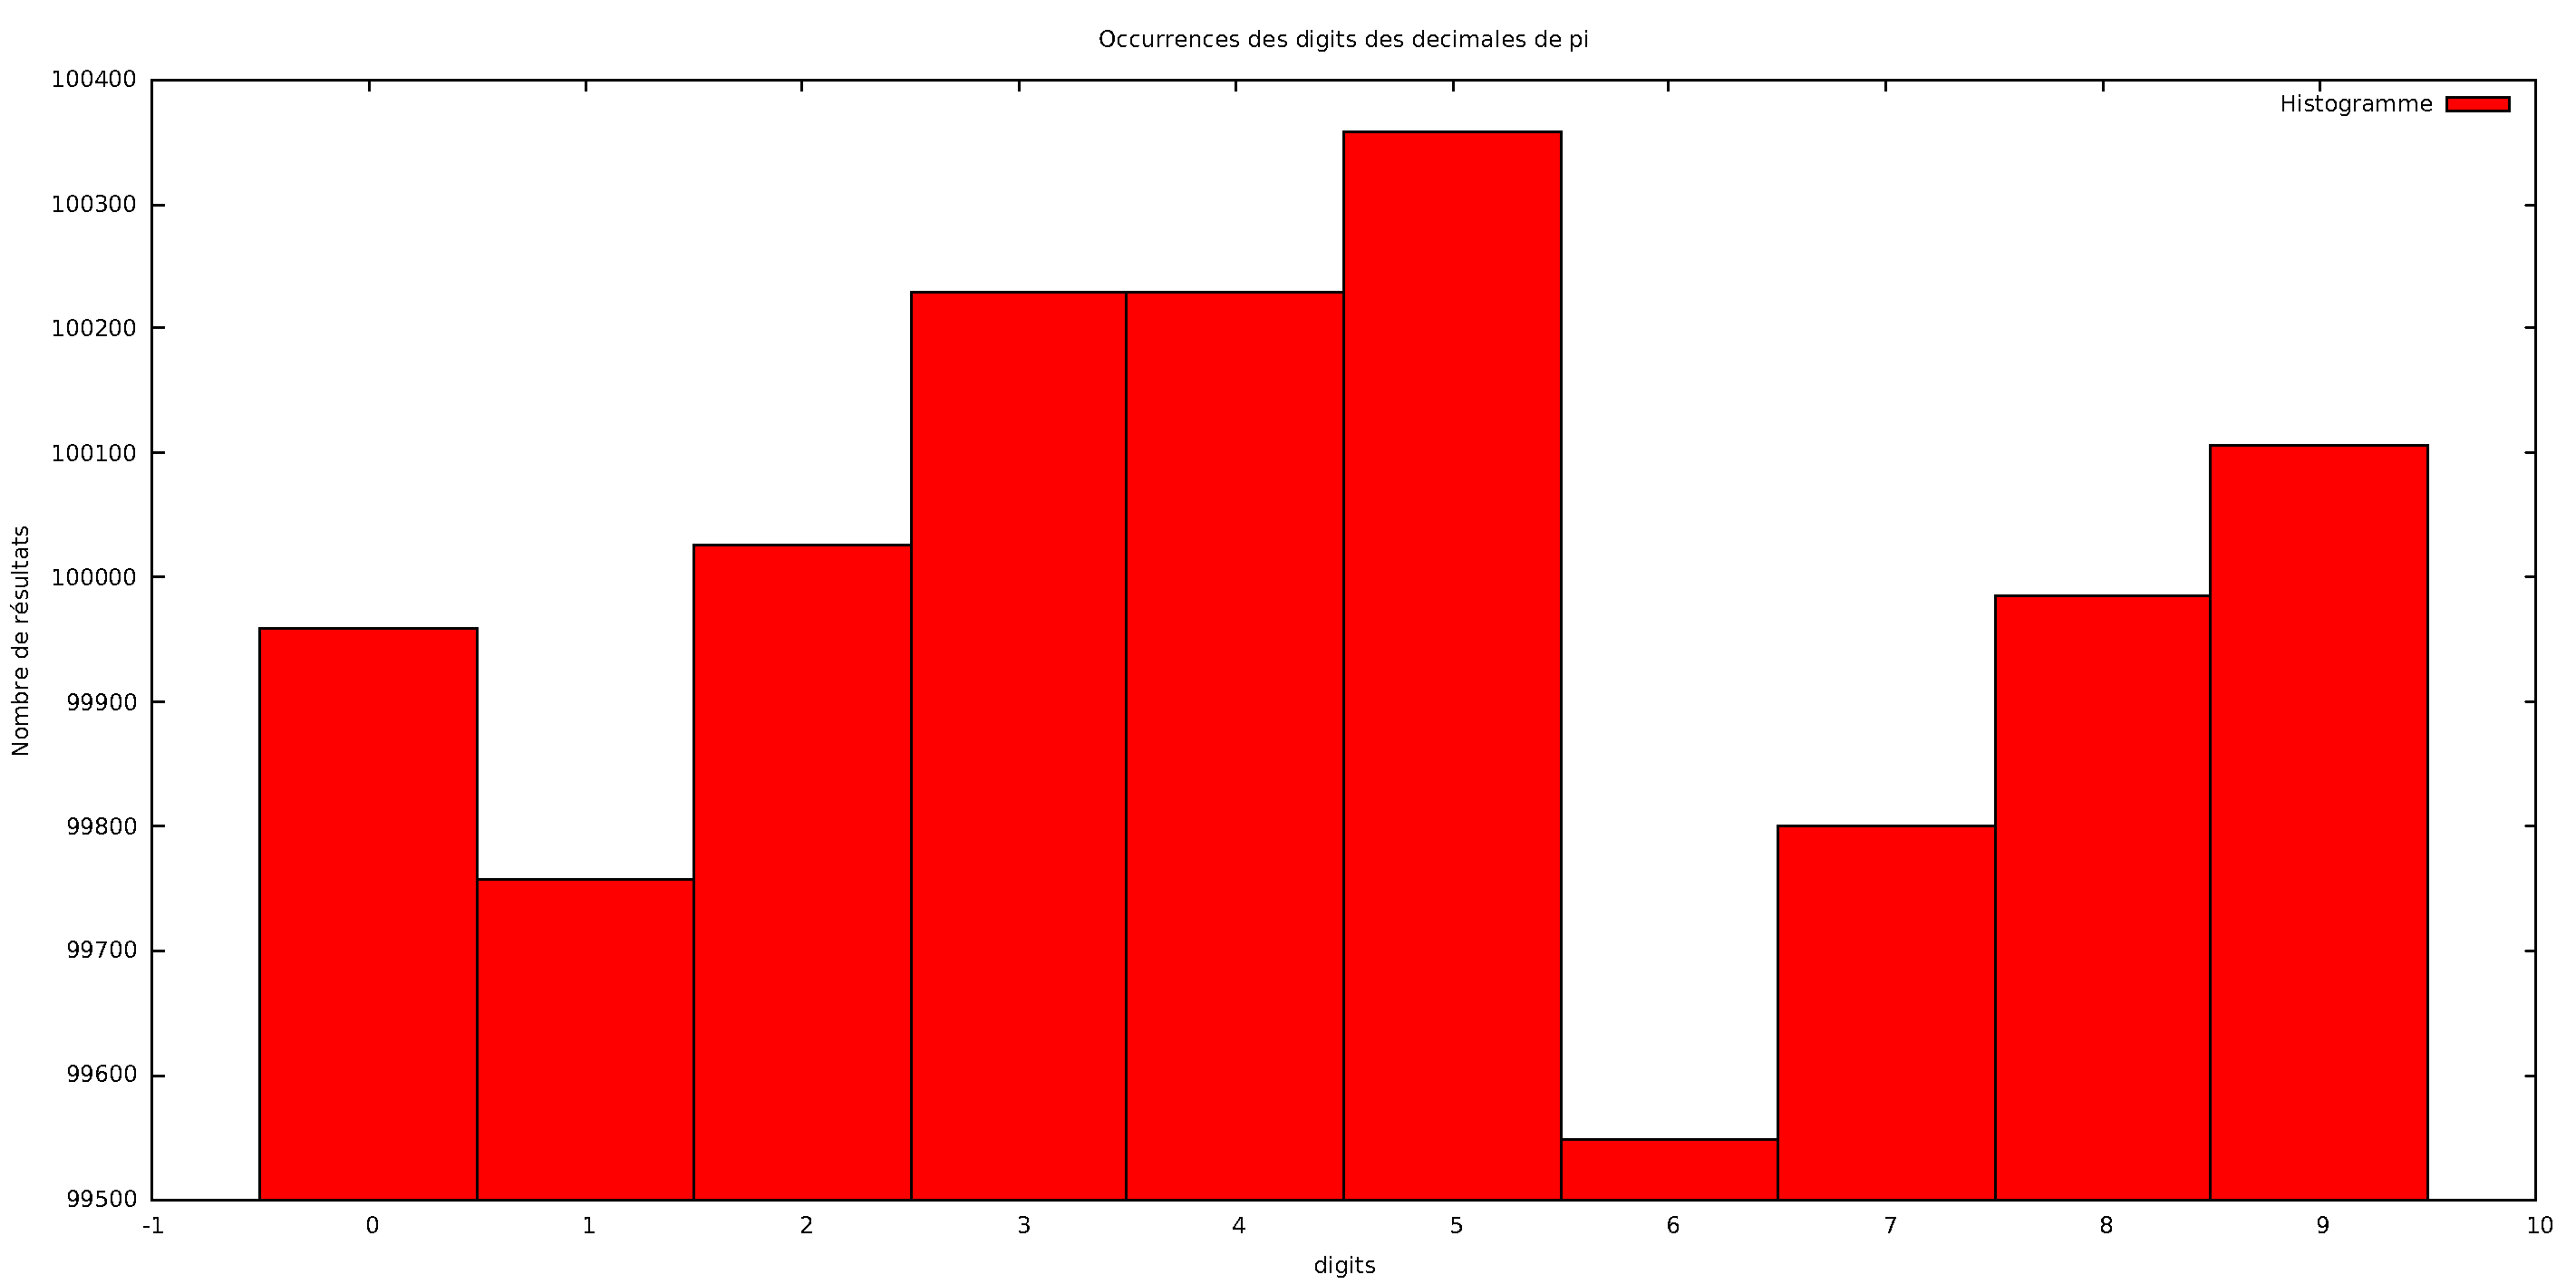
\includegraphics[scale=0.30]{SimuProjet/Archives/Images/histo_zoom}
\end{center}

Mettons désormais les données sous la forme d'un tableau.

\begin{longtable}{|c|c|c|c|c|c|c|c|c|c|}
	\hline
	& \multicolumn{3}{c|}{\textbf{Résultats}} \\ 
	\hline 
	\textbf{Digit}  & \textbf{Observé} & \textbf{Attendu} & \textbf{Erreur en \%} \\ 
	\hline 
	$$0$$ & 99 959 & 100 000 & 0.041\\ 
	\hline 
	$$1$$ & 99 758 & 100 000 & 0.24\\ 
	\hline 
	$$2$$ & 100 026 & 100 000 & 0.026 \\ 
	\hline 
	$$3$$ & 100 229 & 100 000 & 0.229\\ 
	\hline 
	$$4$$ & 100 230 & 100 000 & 0.230\\ 
	\hline 
	$$5$$ & 100 359 & 100 000 & 0.359\\ 
	\hline 
	$$6$$ & 99 548 & 100 000 & 0.452\\ 
	\hline 
	$$7$$ & 99 800 & 100 000 & 0.2\\ 
	\hline 
	$$8$$ & 99 985 & 100 000 & 0.015\\ 
	\hline 
	$$9$$ & 100 106 & 100 000 & 0.106\\ 
	\hline
\end{longtable}

On peut constater qu'entre les résultats observés et attendus, il y a à chaque fois une
erreur inférieur à 0,5\%
\\
Ce qui nous encourage à penser que nos données suivent bien une loi uniforme même si cela ne 
constitue pas une preuve.
\\
Nous allons bientôt passer à l'étude du caractère pseudo-aléatoire des décimales de $\pi$
par l'intermédiaire de 3 tests différents.
\\
\subsection{Test de $\chi^{2}$ }
Le premier test que nous allons effectuer est le test du \textbf{$\chi^{2}$}. Ce dernier est un test statistique qui va permettre de vérifier si une série de données est susceptible de suivre une loi de probabilité.
\\
Pour effectuer ce test, nous allons devoir regrouper ces données dans différentes classes.
Voici un rappel théorique :

	\begin{center}
		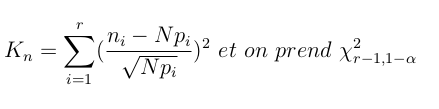
\includegraphics[scale=0.60]{SimuProjet/Archives/Images/khi2}
	\end{center}
	
On peut y apercevoir \textit{r} qui correspond au nombre de classes. \\
\textit{N$p_{i}$} qui correspond aux nombres d'occurrences théoriques. \\
\textit{$n_{i}$} qui correspond aux nombres d'occurrences observées.
\\
\\
Partons désormais de notre hypothèse nulle nommée $H_{0}$ = {nos décimales de $\pi$ suivent une loi uniforme}.
\\
Dans notre cas, \textit{r} sera fixé à 10, car nous considérerons une classe par digit, et \textit{N$p_{i}$} sera fixé à 100 000.\\ 
Quant à \textit{$n_{i}$}, ses différentes valeurs seront issues du nombre d'occurrence observés dans l'histogramme présenté précédemment.
Comme le demande le test de \textbf{$\chi^{2}$}, nous devons fixer une probabilité $\alpha$, appeler erreur de première espèce, de rejeter l'hypothèse nulle $H_{0}$.
\\
Une fois ce paramètre $\alpha$ fixé, nous pouvons désormais vérifier si $H_{0}$ est acceptée
si $K_{n}$ <= $\chi^{2}_{9,\alpha-1}$ où 9 est le degré de liberté calculé en faisant \textit{r}-1 (nombre de classes -1).

Voici les différents résultats obtenus en fonction de différentes valeurs pour $\alpha$.
\\
\begin{longtable}{|c|c|c|c|c|c|c|c|c|c|}
	\hline
	& \multicolumn{3}{c|}{\textbf{Résultats}} \\ 
	\hline 
	\textbf{$\alpha$}  & $K_{n}$ & $\chi^{2}_{9,\alpha-1}$ & \textbf{Resultat} \\ 
	\hline 
	$$0.001$$ & 5.50908 & 27.877 & Reussite\\ 
	\hline 
	$$0.025$$ & 5.50908 & 19.023 & Reussite\\ 
	\hline 
	$$0.1$$ & 5.50908 & 14.684 & Reussite \\ 
	\hline 
\end{longtable}

On peut constater que les tests réussis, nous sommes donc confortés dans notre supposition qui était que les décimales de $\pi$ suivent une loi uniforme.
\\

\end{document}
